\documentclass[10pt]{beamer}
\usetheme{default}

\usepackage[absolute,overlay]{textpos}
\usepackage{fancyvrb}

\title{Architektur und Modellierung}
\author{}
\date{}

\beamertemplatenavigationsymbolsempty
\setbeamertemplate{footline}[frame number]

\begin{document}
\begin{frame}[plain]
    \maketitle
\end{frame}

\begin{frame}{Übersicht}
	\tableofcontents
\end{frame}

\section{Architektur}
\subsection{Architektur?}
\begin{frame}{Clean Architecture}
	\begin{itemize}
		\item SOLID auf Architekturebene: Komponenten anstatt Klassen
		\item ,,Ausführeungsart`` irrelevant: SoA, Pluginarchitektur, \ldots
		\item \textbf{Seperation of Concerns}
		\item Grenzen zwischen Komponenten
		\item Einsatzzweck vermitteln
		\item<2-> Zwecke
		\begin{itemize}
			\item Entscheidungen soweit verzögern wie Nötig
			\item Unterstützen in Entwicklung und Wartung
			\item Reduzierung der Folgekosten, Optionen offen halten
			\item $\rightarrow$ OCP
		\end{itemize}
	\end{itemize}
\end{frame}
\begin{frame}{SOLID auf Architekturebene}
	\begin{itemize}
		\item<+-> \textbf{Common Closure Principle}: Gruppiere Klassen in Komponenten, die sich aus den selben Gründen zur selben Zeit ändern. Separiere Klassen, die dies nicht tun. ($\rightarrow$ SRP)
		\item<+-> \textbf{Common Reuse Principle}: Zwinge Nutzer einer Komponente nicht von Dingen abzuhängen, die nicht benötigt werden. ($\rightarrow$ ISP)
		\item<+-> \textbf{Reuse/Release Equivalence Principle}: Der Grad von Wiederverwendung entspricht dem Grad des Releases. Anders: Klassen einer Komponente sollen kohärent sein.
		\item<+-> \textbf{Acyclic Dependencies Principle}: Verbiete zyklische Abhängigkeiten zwischen Komponenten.
		\item<+-> {\color{gray} \textbf{Stable Dependency Principle} und \textbf{Stable Abstraction Principle}.}
		\item<+-> \textbf{The Dependency Rule}: Quelltextabhängigkeiten zeigen immer in Richtung höherer Regeln (policies)
	\end{itemize}
\end{frame}
\begin{frame}{Clean Architecture: The Dependency Rule}
	\begin{center}
		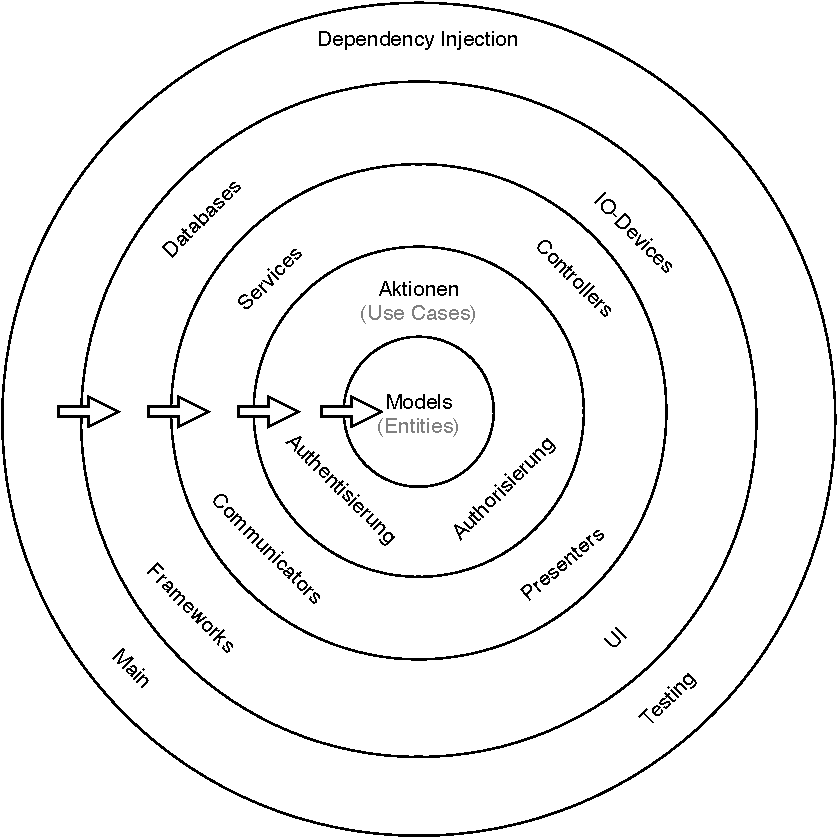
\includegraphics[scale=0.5]{clean-architecture}

		\textbf{The Dependency Rule}: Quelltextabhängigkeiten zeigen immer in Richtung höherer Regeln (policies)
	\end{center}
\end{frame}
\begin{frame}{Details}
	\begin{itemize}
		\item Die Datenbank ist ein Detail.
		\item Das Web ist ein Detail (IO-Device)
		\item Frameworks sind Details
	\end{itemize}
\end{frame}

\subsection{OpenSlides 3}
\begin{frame}{Wieso Neuschreiben?}
	\begin{itemize}
		\item Zu starke Kopplung in Django/DRF. Verstöße gegen die Abhängigkeitsregel, \ldots
		\item ORM bietet nicht die Möglichkeit zur Versionierung
		\item REST-Schnittstelle ist nicht für Aktionen geeignet
		\item Autoupdate zu groß
		\item Cache-Ansatz nicht skalierbar für neue Anforderungen
		\item<2-> Was bleibt übrig?
	\end{itemize}
\end{frame}
\begin{frame}{Keine Microservices}
	\begin{itemize}
		\item Architektur hält diese Entscheidung offen
		\item Trennen nach Apps führt zu zyklischen Abhängigkeiten
		\item Viele geteilte Belange; Transaktionen?
	\end{itemize}
	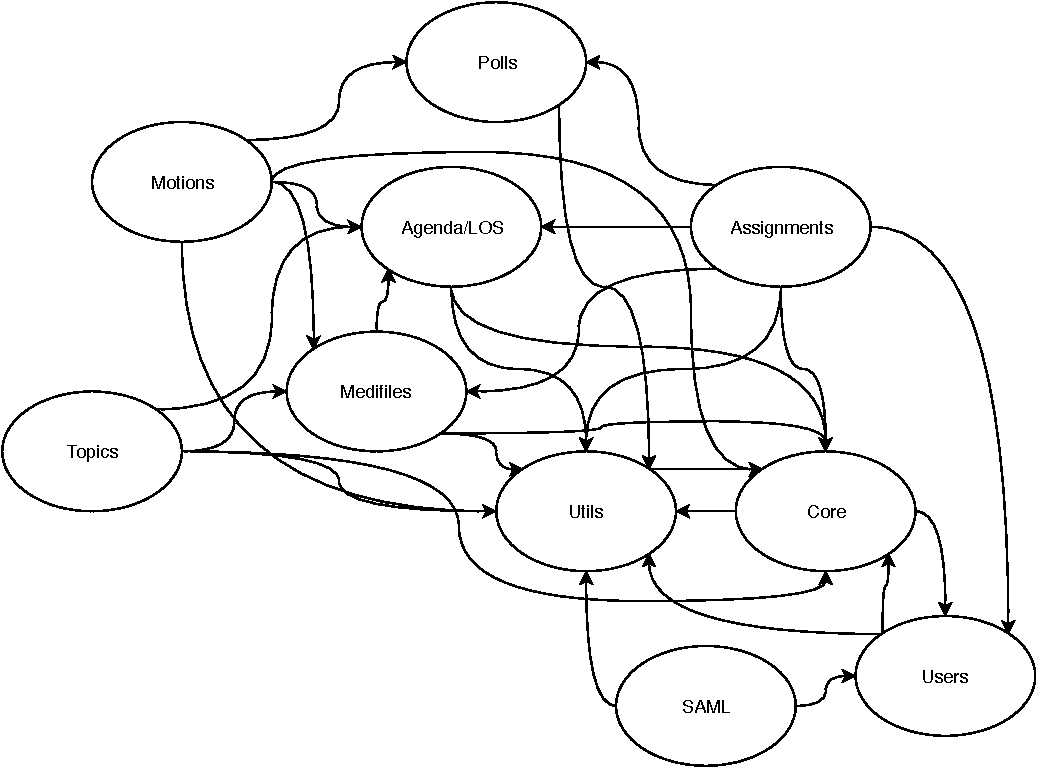
\includegraphics[scale=0.5]{os3-modelle}
\end{frame}

\subsection{Zerlegung in Belange}
\begin{frame}{Separation of Concerns}
	Was sind unsere Belange?
	\begin{enumerate}
		\item Businessregeln
		\item Authorisierung
		\item Authentisierung
		\item Persistenz (inkl. Versionierung)
		\item Echtzeit-Updates
	\end{enumerate}
	\pause
	Geteilte Belange
	\begin{enumerate}
		\item Cache
		\item Logging
		\item Konfiguration der Software
	\end{enumerate}
	\pause
	$\Rightarrow$ Teilen der Belange in Komponenten
\end{frame}
\begin{frame}{Separation of Concerns: Ein Versuch}
	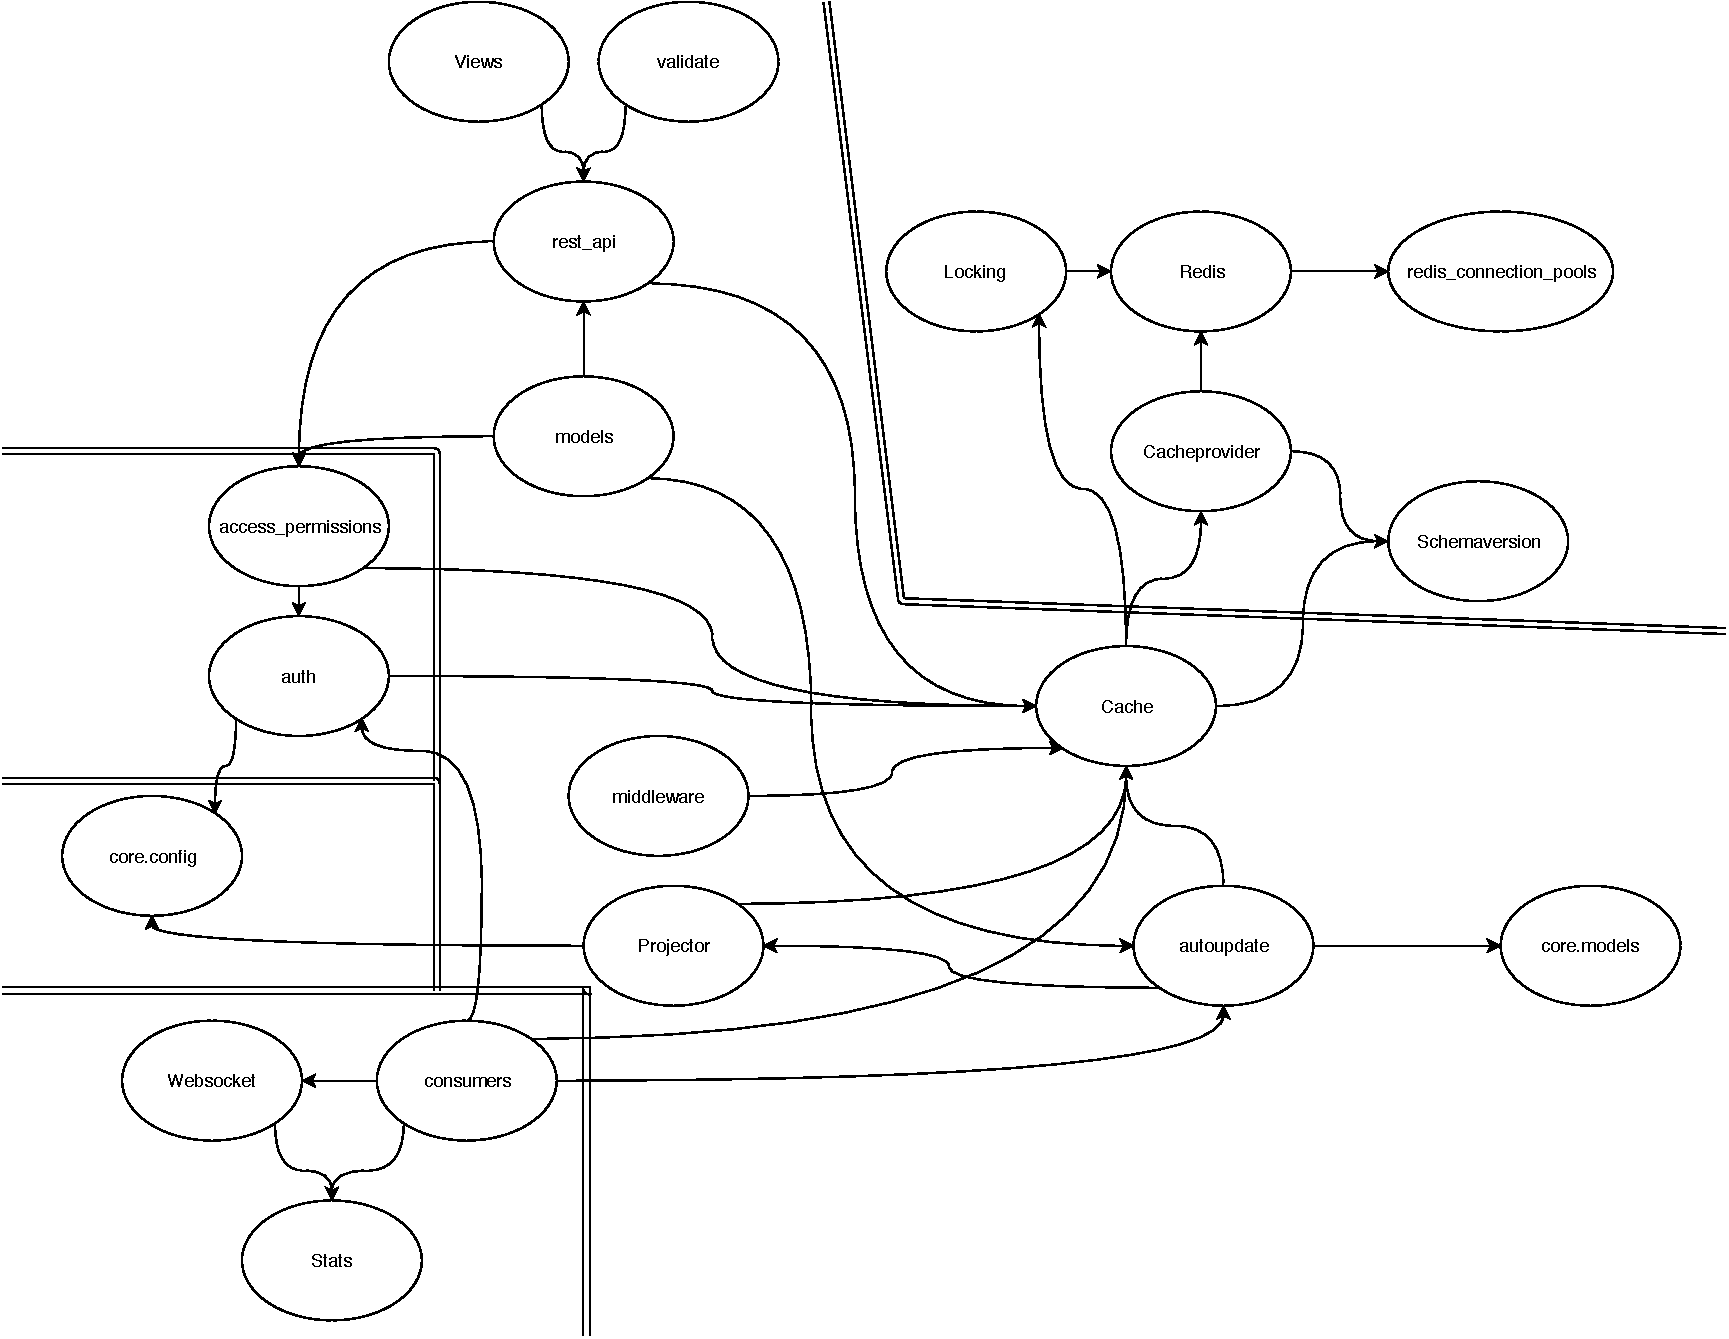
\includegraphics[scale=0.38]{os3-module}
	\begin{textblock*}{7.3cm}(5.3cm,8cm) % {block width} (coords)
		\visible<2->{
		$\Rightarrow$ Teilweise OK!\\
		Einige Abhängigkeiten sind falsch: Wieso muss auth wissen, dass die Daten in einem ,,Cache`` liegen?
		}
	\end{textblock*}
\end{frame}
\begin{frame}{Zerlegung in Komponenten}
	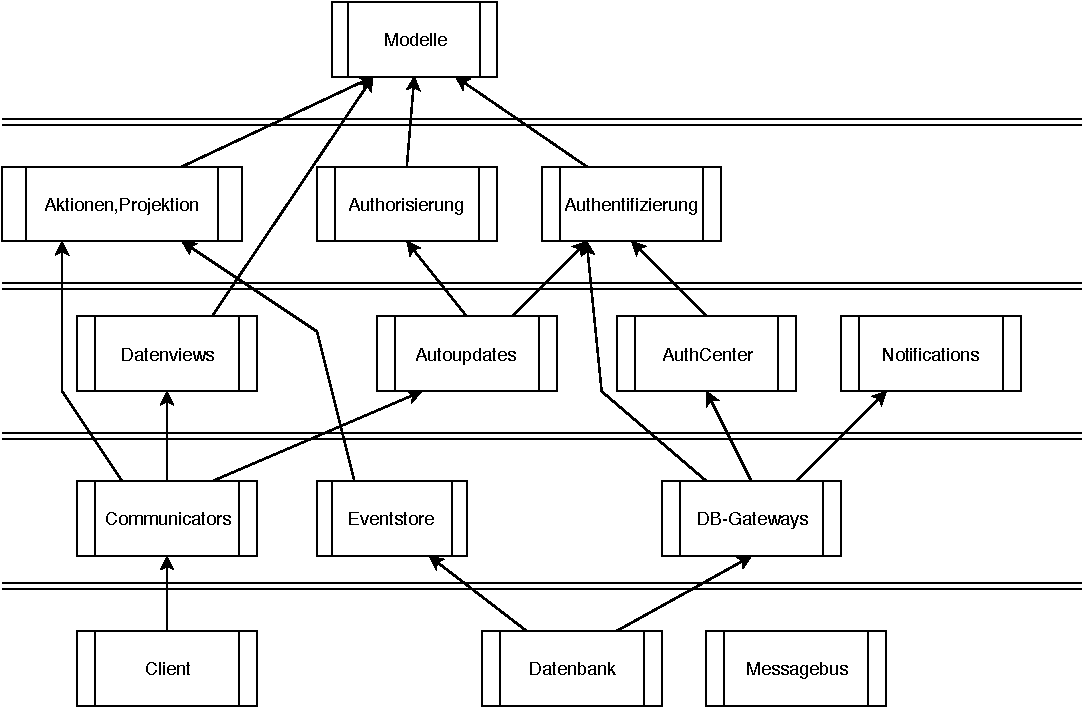
\includegraphics[scale=0.5]{hierachie}
	
	\begin{itemize}
		\item Nicht vollständig (Pfeile sind Quelltextabhängigkeiten)
		\item Hierachie: Oben: Businessregeln, Mitte: Verarbeitung, Unten: IO
	\end{itemize}
\end{frame}
\begin{frame}
	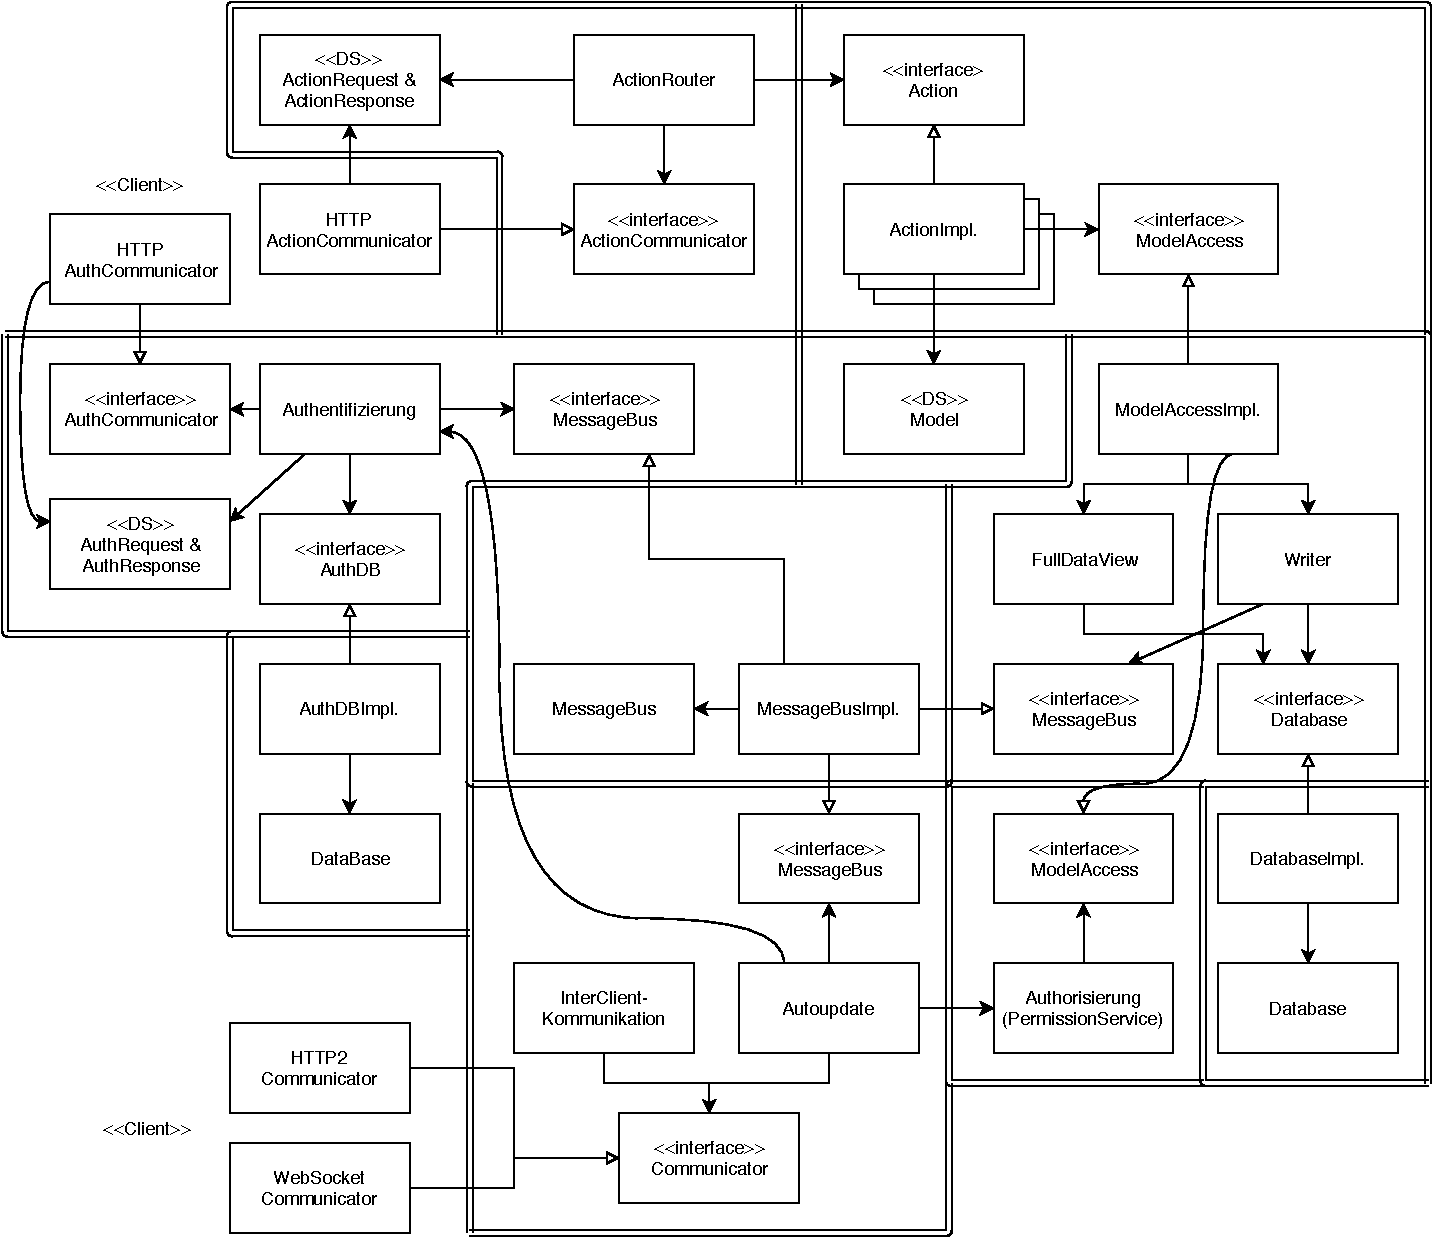
\includegraphics[scale=0.45]{komponenten}
	TODO: Hinweise
\end{frame}
\begin{frame}{Eventsourcing}
	Was ist Eventsourcing?
	\begin{itemize}
		\item Append-only Log an Änderungen (Events)
		\item Repräsentation des Systemzustandes
		\item Wiederherstellung durch Abspielen der Events
		\item Snapshots für beschleunigte Wiederherstellung
		\item siehe GIT
	\end{itemize}

	\visible<2>{
	Eigenschaften:
	\begin{itemize}
		\item Kann als ,,Persistenz mit Versionierung`` abstrahiert werden
		\item Bietet folgenden Vorteil: CRUD $\rightarrow$ CR
		\item Ermöglicht funktionale Programmierung für Aktionen: EVA
		\item Erinnerung: SSOT
		\item Eventstore ist Implementation der ,,Persistenz mit Versionierung`` mit Eventsourcing
	\end{itemize}
	}
\end{frame}

\subsection{Services?}
\begin{frame}{Wieso Services?}
	\begin{itemize}
		\item Entkopplung auf \textit{Quelltext-Level}, \textit{Komponenten-Level}, \textit{Service-Level}
		\item OS3: Misch aus Quelltext- und Komponenten-Level
		\item Erfahrung: Unterschiedlichste Anforderungen an verschiedene Teile des Systems
		\item<2-> SoA: Teilung nach Belangen (deren Anforderungen), nicht nach Komponenten
		\item<2-> Services selbst sollen auf Komponenten-Level sein
		\item<3-> Vorteile?
		\begin{itemize}
			\item Wiederverwendbarkeit?
			\item Unabhängigkeit?
			\item<4-> Testbarkeit!
			\item<4-> Anpassungsfähigkeit! (Ressourcenmanagement)
			\item<4-> Stärkste Trennung der Belange! 
		\end{itemize}
	\end{itemize}
\end{frame}

\subsection{Details}
\begin{frame}{Details}
	\ldots sind für die Architektur irrelevant! Jedoch für die Erstimplementation:
	\begin{itemize}
		\item<2-> Bedachte Wahl von Technologien: Jede eingesetzte Technologie muss \textbf{verstanden} und \textbf{beherrscht} werden können
		\item<3-> Je größer die Vielzahl an Protokollen, Datenbanken, Caches,\ldots, je komplexer wird die Software
		\item<4-> Kapseln von Technologien: Unser Code ist unabhängig von diesen!
		\item<5-> Vorgabe: Postgresql für jegliche Persistenz\\
		\textbf{Achtung}: Das bedeutet nicht, dass keine Abstraktion stattfindet ($\rightarrow$ Testen)
	\end{itemize}
\end{frame}

\section{Services}
\begin{frame}
\begin{center}
	\usebeamerfont{title}\usebeamercolor[fg]{title}Services
\end{center}
\end{frame}
\subsection{Übersicht}
\begin{frame}{Übersicht}
	\hspace*{-0.9cm}
	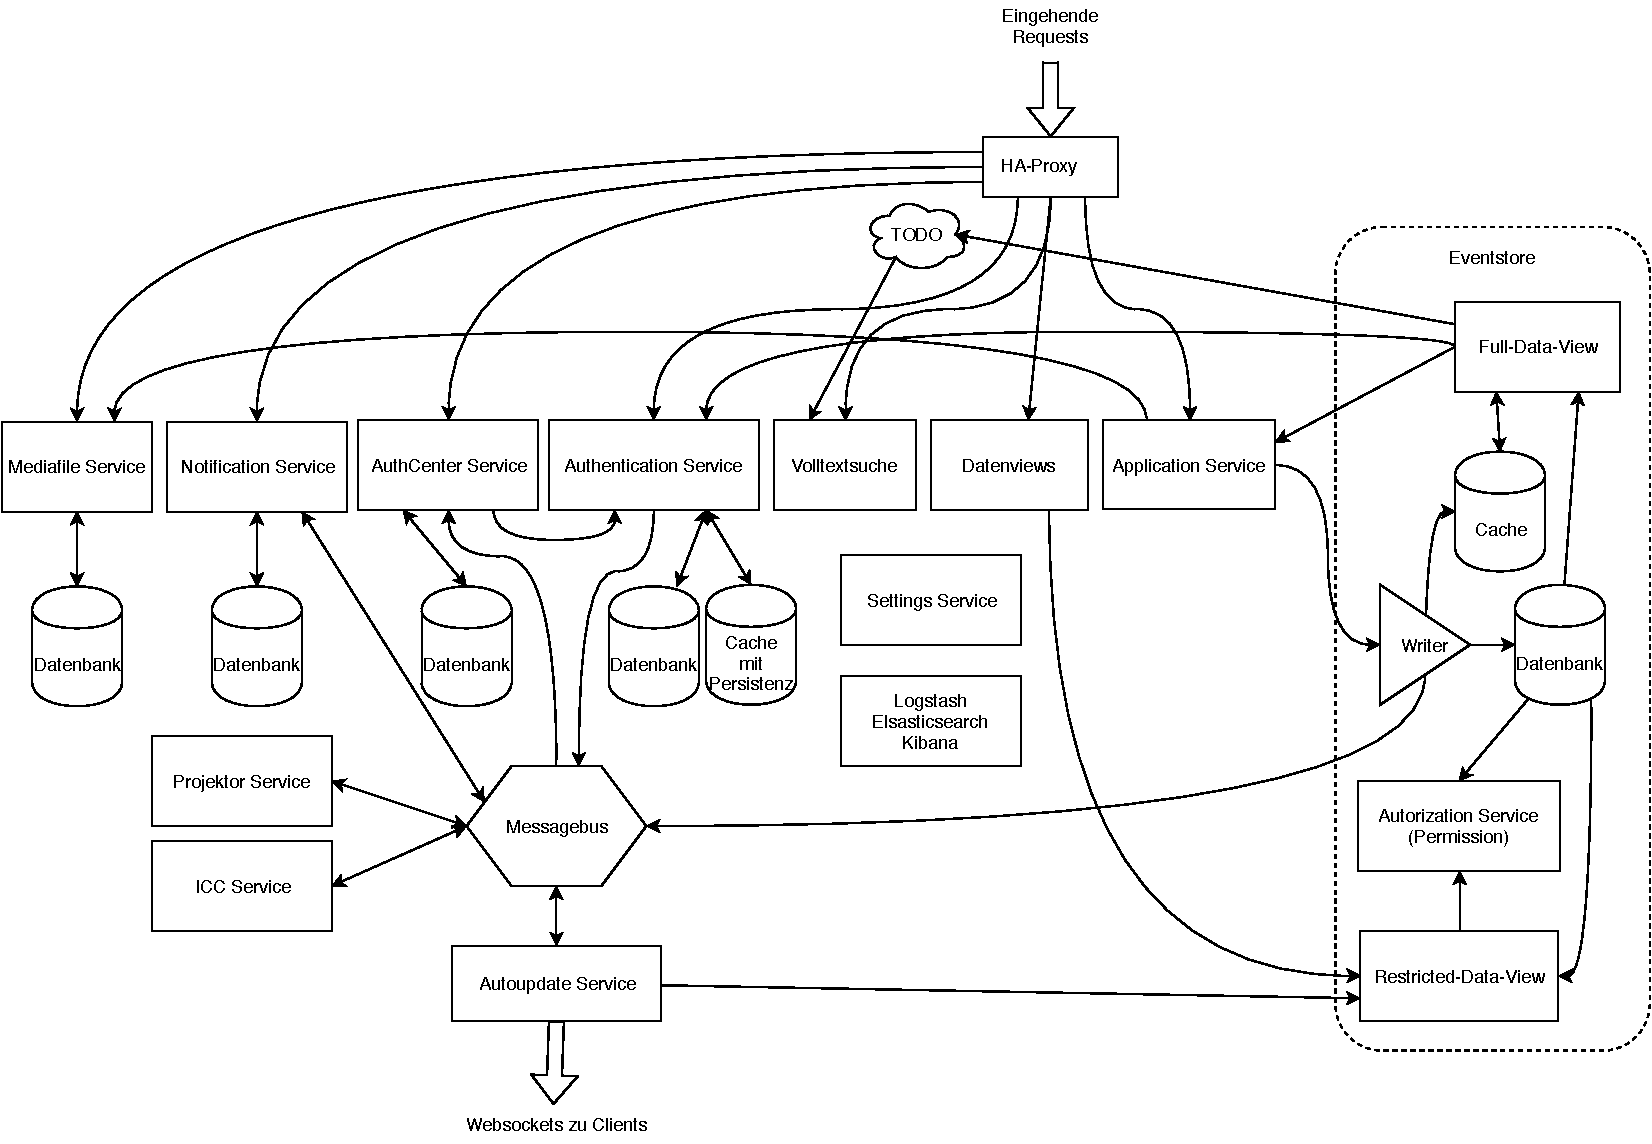
\includegraphics[scale=0.45]{services}
	\begin{textblock*}{5cm}(1cm,1.4cm) % {block width} (coords)
		{\color{gray} (Pfeile entsprechen Kontrollfluss)}
	\end{textblock*}
\end{frame}

\subsection{Modelle}
\begin{frame}{Modelle}
	\small
	\begin{itemize}
		\item<+-> Ansammlung an Key-Value-Paaren
		\item<+-> Orientiert an OS3
		\item<+-> Dokumente, Verschachtelung möglich, aber nicht erwünscht
		\begin{itemize}
			\item Autoupdates und Events sind auf Key-Basis
			\item Keine Notwendigkeit der Denormalisierung durch Verschachtelung
		\end{itemize}
		\item<+-> Referenzen werden in beiden Modellen gespeichert: Vereinfachtes Lesen 
		\item<+-> IDs: Nur Zahlen?
		\item<+-> Keys bestehen aus \texttt{[a-z\_]+}
		\item<+-> Struktur innerhalb der Keys durch \texttt{:} (\texttt{amendment\_paragraphs:3}, \texttt{meta:position})
		\item<+-> Reservierter meta-Key-Prefix: Position des Modells, gelöscht,\ldots (später)
		\item<+-> Modelle sind Collections zugeordnet: \texttt{motions}, \texttt{projector}, \texttt{motion-state},\ldots
		\item<+-> \textit{fqid} (full-qualified-id): \texttt{<collection>/<id>}, z.B.: \texttt{projector-message/42}
		\item<+-> \textit{fqkey} (full-qualified-key): \texttt{<fqid>/<key>}, z.B.: \texttt{projector-message/42/message}
		\item<+-> String-values: HTML-Strings bekommen eine Maximallänge (konfigurierbar, TODO: Wo?)
	\end{itemize}
	\normalsize
\end{frame}

\subsection{Eventstore}
\begin{frame}{Eventstore}

	{\color{gray}AKA. Transaction log, Incremental Backup,\ldots}\\[5mm]
	Datenfelder von Events
	\begin{enumerate}
		\item Event-Id: Intern.
		\item Position: Totale Ordnung, bündelt zusammengehörige Events.
		\item fqid: Jedes Event ist einem Modell zugeordnet
		\item Eventtyp
		\begin{itemize}
			\item Create
			\item UpdateKeys
			\item DeleteKeys
			\item Delete
			\item Restore
			\item Noop (Intern)
		\end{itemize}
		\item Eventdaten als partielles Modell
		\item Schemaversion
		\item Zuordnung von Zeitstempel, Beschreibung,\ldots zu Position
		\item Benötigt: Zuordnung Veranstaltung $\leftrightarrow$ Modell?
	\end{enumerate}
\end{frame}
\begin{frame}{Eventstore}
	Methoden
	\begin{itemize}
		\item Schreiben von Events
		\begin{itemize}
			\item 
		\end{itemize}
		\item Single-Writer: Keine Synchronisation nötig, ist atomar
		\item Konsistenz der Events wird abgesichert.
		\item OCC: ,,Lazy`` Isolation
		\item $\rightarrow$ ACID
	\end{itemize}
\end{frame}
\begin{frame}[fragile]{Beispiel: Eventstore write}
	\footnotesize
	\begin{Verbatim}[tabsize=2]
	write(request: WriteRequest): WriteResponse;
	
	Interface WriteRequest{
		data: {
			<fqid>: {position: Position; type: Create|Restore; model: Model;}
				| { position: Position; type: Delete;};
			<fqkey>: {position: Position; type: Update; value: any;}
				| { position: Position; type: DeleteKey;};
		};
		general_keys: {
			<CollectionKey>: Position; // TODO: je nach dem wie IDs aussehen (nur
			// Zahlen?) ist CollectionKey nicht eindeutig von fqid zu unterscheiden
			<fqid>: Position;
			<fqkey>: Position;
		};
	}
	
	Interface WriteResponse{
		changed_models: {<fqid>: Position};
		current_position: Position;
	}
	\end{Verbatim}
\end{frame}
\begin{frame}{Beispiel: Eventstore write}
	Wirft Exceptions:
	\begin{itemize}
		\item ModelDoesNotExist(fqid)
		\item ModelTooOld(fqid)
		\item KeyTooOld(fqkey)
		\item RequestTooOld()
		\item ModelExists(fqid); Kann bei Create auftreten, wenn die ID bekannt ist.
	\end{itemize}
	\pause
	Weiteres:
	\begin{itemize}
		\item Besonderheit: ID muss bei Create bekannt sein. Der Aufrufer muss sich darum kümmern.
		\item Vorteil: Relations können bei Create angelegt werden
		\item<3-> Single Writer: Keine Synchronisation nötig
		\item<4-> OCC: Eine Datenstruktur hält die letzten $X$ geänderten fqids/fqkeys
		\item<5-> Beispiel: Create mit unique Key
	\end{itemize}
\end{frame}

%\begin{frame}{Beispiel: Eventstore read}
%	Muss getan werden
%\end{frame}

\begin{frame}{Papierkorb}
	\begin{itemize}
		\item Elemente lassen sich wiederherstellen
		\item DSGVO: Wir (als Betreiber) können in die Datenbank des Eventstores eingreifen und z.B. Nutzer entfernen (d.h. nicht das Nutzer-Model löschen, sondern Daten unkenntlich machen)
		\item Wiederherstellung benötigt Logik für alle Referenzen
		\begin{itemize}
			\item Existieren diese noch?
			\item Falls Ja, sind diese valide? $\rightarrow$ Beide Modelle anpassen (doppelte Referenzen)
			\item Falls Nein, ist das valide?
			\item Falls nicht valide: Nutzer bekommt "Create"-Form zum Bearbeiten
		\end{itemize}
	\end{itemize}
\end{frame}

\subsection{Aktionen}
\begin{frame}{Aktionen}
	\begin{itemize}
		\item Atomar
		\item Hat Bezeichner. Z.B.: \texttt{motions/reset-state}, \texttt{user/add\_group},\ldots
		\item Input: \texttt{data: Object} und \texttt{user\_id: ID}
		\item Output: \texttt{events: Event[]}
		\item Aktionen teilen sich in \texttt{validate} und \texttt{execute}
		\item Client kann mehrere Aktionen schicken. Ausführungsmodi:
		\begin{itemize}
			\item Sukzessive bearbeiten; Nach Validierung sofort ausführen; Beim ersten Fehler abbrechen\\
			($\rightarrow$ Operationen, die aufeinander aufbauen, aber in Summe nicht atomar sind)
			\item Sukzessive bearbeiten; Nach Validierung sofort ausführen; Alle Fehler melden\\
			($\rightarrow$ unabhängige Operationen, z.B. Bulk-Operationen)
			\item Erst alle Validieren, dann alle Ausführen\\
			($\rightarrow$ Transaktion; Single-Writer versichert atomare Ausführung)
		\end{itemize}
		\item Autoupdate in Response
	\end{itemize}
\end{frame}

\subsection{Autoupdates}
\begin{frame}[fragile]{Autoupdates}
	\begin{itemize}
		\item \textit{Fokussierte} Modelle (Detail/Liste)
		\item Client abonniert fokussierte Modelle inkl. benötigter Keys (ID implizit) und Relationen
	\end{itemize}
	\begin{Verbatim}[tabsize=2]
	interface ModelDescriptor {
		<key>: ModelDescriptor | null;
		// null -> Nur der Wert des Keys
	}
	
	interface ModelRequest {
		ids: number | number[] | null;
		// Ein spezifisches Modell, mehrere spezifische Modelle
		// oder alle Modelle (siehe assembly_id)
		assembly_id: number | null; // Benötigt für ids=null
		collection: string;
		keys: ModelDescriptor;
	}
	\end{Verbatim}
\end{frame}
\begin{frame}[fragile]{Autoupdates: Beispiel}
	\footnotesize
	\begin{columns}
		\begin{column}{0.48\textwidth}
			\begin{Verbatim}[tabsize=2]
			modelRequest = {
				ids: 4,
				collection: 'motion-workflow',
				keys: {
					name: null,
					states_id: null,
					first_state_id: {
						collection: 'motion-state',
						keys: {
							name: null,
							css_class: null,
							next_states_id: {
								name: null
							}
						}
					}
				}
			}
			\end{Verbatim}
		\end{column}
		\begin{column}{0.48\textwidth}  %%<--- here
			\begin{Verbatim}[tabsize=2]
			ExampleDataFromServer = {
				'motion-workflow': {
					4: {
						name: 'Example Workflow',
						states_id: [1,2,3,4,5,6],
						first_state_id: 1,
					}
				},
				'motion-state': {
					1: {
						id: 1,
						name: 'My first state',
						css_class: 'lightblue',
						next_states_id: [2, 3]
					},
					2: {
						id: 2,
						name: 'Accept'
					},
					3: {
						id: 2,
						name: 'Deny'
					}
				}
			}
			\end{Verbatim}
		\end{column}
	\end{columns}
\end{frame}
\begin{frame}{Autoupdates}
	\begin{itemize}
		\item Jede Subscription hat ein Handle zum Beenden
		\item Kein Caching (vorerst)
		\item Client übernimmt Flusssteuerung; Server kann Autoupdates akkumulieren
		\item TODO: Vorsätzliche Akkumulierung?
		\item TODO: Explizites vs. Implizites Abonnieren im Client
	\end{itemize}
\end{frame}


\subsection{Weiteres}
\begin{frame}{Weiteres}
	\begin{itemize}
		\item Offlinemodus: Explizit anstatt Implizit
		\item Presenters
		\item Mediafiles: Speichern in einer Datenbank. Extra Service zum Ausliefern
		\item Im- und Export von Veranstaltungen
		\item Volltextsuche: ?
		\item Migrationen: ?
		\item Einstellungen
		\item Logging
	\end{itemize}
\end{frame}

\section{Modellierungen}
\begin{frame}
	\begin{center}
		\usebeamerfont{title}\usebeamercolor[fg]{title}Modellierungen
	\end{center}
\end{frame}
\begin{frame}{ER-Diagramm für Organisationsebene}
	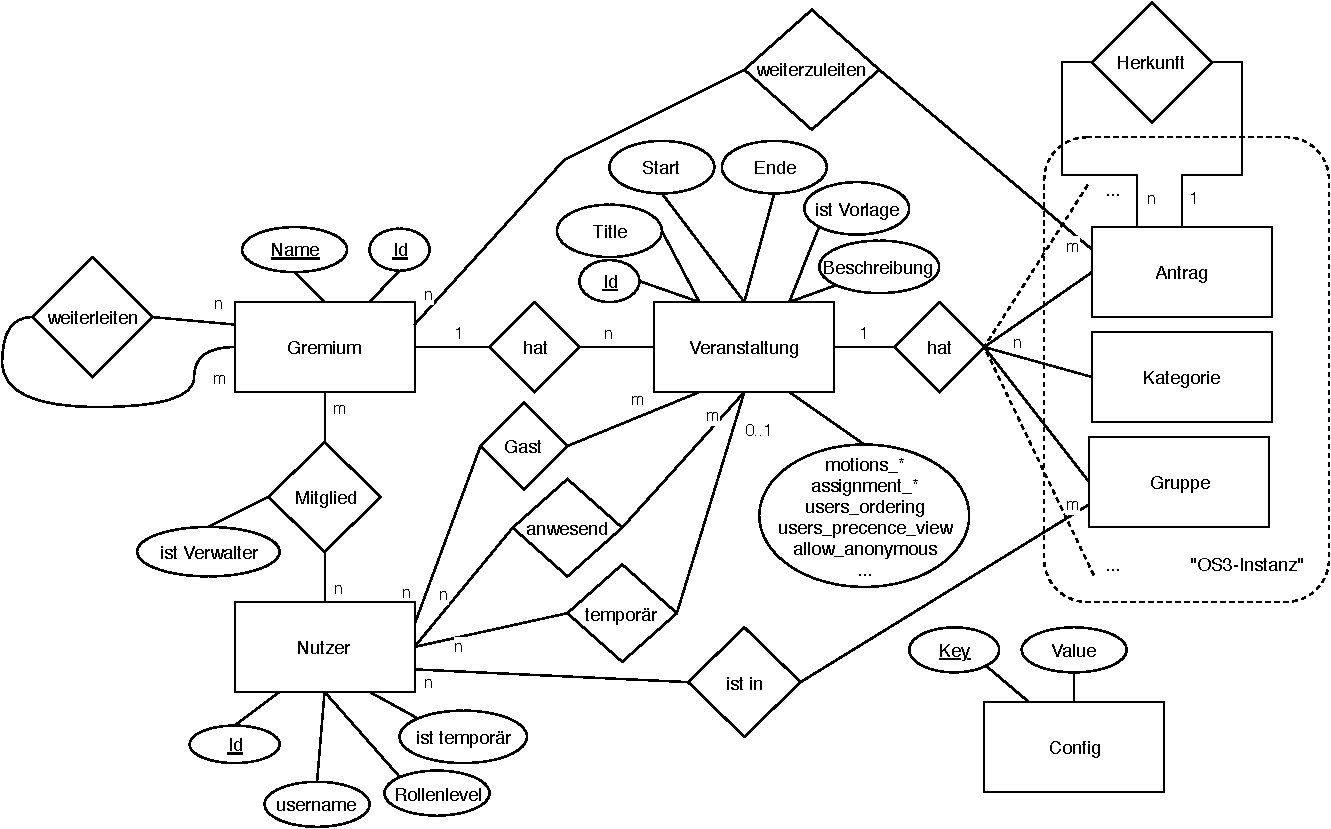
\includegraphics[scale=0.5]{modellierung}
\end{frame}
\begin{frame}{Rollen auf Organisationsebene}
	\begin{itemize}
		\item Rollenlevel:
		\begin{enumerate}
			\setcounter{enumi}{-1}
			\item \textbf{Keine Berechtigungen} (Standard): Ein Nutzer darf die Gremien sehen, in der er Mitglied ist, oder in einer Veranstaltung Gast
			\item \textbf{Nutzer-Manager}: Darf Nutzer verwalten (erstellen, temporär zu fest, bearbeiten, Löschen, Passwort managen, sperren)
			\item \textbf{Organisations-Manager}: Nutzer-Manager + Darf alle Gremien sehen, erstellen, löschen, Nutzer zuweisen, Nutzer als Verwalter im Gremium ernennen und die Weiterleitungsstruktur bearbeiten
			\item \textbf{Superadmin}: Wie Organisations-Manager, hat jedoch in allen Gremien und Veranstaltungen alle Rechte (transitiv)
		\end{enumerate}
		\item<2-> Jeder darf eigene Rolle ändern, aber nur abstufen
		\item<3-> Ab Rollenlevel $L\geq1$ darf ein Nutzer andere Rollenlevel setzten, aber nur auf maximal $L$
		\item<4-> Es existiert immer ein Superadmin
	\end{itemize}
\end{frame}
\begin{frame}{Rollen in Gremien}
	\begin{itemize}
		\item \textit{Mitglieder} sind dem Gremium zugeordnete Nutzer
		\item Mitglieder sehen Veranstaltungen, die Anonymous erlauben, der Nutzer Gast ist, oder der Nutzer in mindestens einer Gruppe ist
		\item Mitglieder können Verwalter sein
		\item Superadmins auf Organisationsebene sind implizit Mitglied und Verwalter
		\item Verwalter können Veranstaltungen verwalten: Erstellen, Löschen, Kopieren, Vorlage auswählen, Importieren, Exportieren, Eigenschaften der Veranstaltung ändern
		\item<2-> Nutzer, die Gäste aber keine Mitglieder sind, sehen Gremien nicht
		\item<2-> Im Dashboard gibt es eine Übersicht von Veranstaltungen, in denen ein Nutzer Gast ist
		\item<3-> Veranstaltungen können optionalen eindeutigen Identifikator erhalten (Gäste können darüber zugreifen)
	\end{itemize}
\end{frame}
\begin{frame}{Berechtigungen in Veranstaltungen}
	\begin{itemize}
		\item Rechte auf Basis der Gruppenzuweisung
		\item Es gibt eine Gästegruppe für Gäste ($\hat{=}$ Default in OS3)
		\item Es gibt eine Superadmingruppe
		\item Superadmins auf Organisationsebene sind implizit in der Superadmingruppe
		\item Gremienverwalter sind implizit in der Superadmingruppe
		\item Nutzer mit \texttt{users.can\_manage} können Nutzer Gruppen zuweisen und Gruppenberechtigungen einstellen
		\item Nutzer bekommen neues Feld "Funktion", damit die Gruppen nur für die Rechtezuweisungen benutzt werden
	\end{itemize}
\end{frame}
\begin{frame}{URLs}
	\begin{itemize}
		\item Veranstaltungen:\\\texttt{org.openslides.com/<assembly\_id>/}
		\item Veranstaltungen mit eindeutigem Identifikator: \texttt{org.openslides.com/<identificator>/}
		\item Serverkonfiguration (HaProxy, optional): \texttt{<identificator>.org.openslides.com/}
		\item<2-> Dashboard (als main landing page) unter \texttt{org.openslides.com/}
		\item<2-> Spezielle URLs: \texttt{/dashboard/}, \texttt{/users/}, \texttt{/committee/}, \texttt{/auth/}
		\item<2-> Spezielle Urls könen nicht als Identifikatoren verwendet werden
	\end{itemize}
\end{frame}
\begin{frame}{Anonymous}
	\begin{itemize}
		\item Anonymous $\leftrightarrow$ Gast
		\item Kann pro Veranstaltung aktiviert werden
		\item Sind implizit in der Gästegruppe
		\item Anonymous sehen nicht das Dashboard und Gremien
		\item Müssen Veranstaltungs-URL kennen
	\end{itemize}
\end{frame}
\begin{frame}{Temporäre Nutzer}
	\begin{itemize}
		\item Szenario:
		\begin{itemize}
			\item Nutzergruppe der Veranstaltung nicht bekannt
			\item Anwesende Nutzer sollen in OpenSlides teilnehmen
			\item Einen systemweiten Nutzer anzulegen ist keine Option
		\end{itemize}
		\item<2-> \texttt{users.can\_manage\_temporary\_user}
		\item<3-> Im System sind dies normale Nutzer, haben jedoch eine \texttt{assembly\_id} (\texttt{temporär := assembly\_id != null})
		\item<4-> Temporäre Nutzer können sich einloggen, wenn Passwort vergeben (optional!)
		\item<5-> Temporäre Nutzer können gelöscht werden.
		\item<6-> In zentraler Nutzerverwaltung: Vereinigung temporärer Nutzer und umwandlung in systemweiten Nutzer (\texttt{assembly\_id=null})
	\end{itemize}
\end{frame}

\end{document}
